\documentclass[12pt, a4paper, oneside]{article}
\usepackage[headheight=0.3in, headsep=0.2in, hmargin={1.2in,1in}, vmargin={1in,1in}]{geometry}
\textwidth 16.5 cm \textheight 24cm
% \oddsidemargin -2mm

% Packages
\usepackage{amsmath, physics, listings, xcolor, tcolorbox, microtype, fancyhdr, hyperref, tikz, float, pgfplots}
\usetikzlibrary{decorations.pathreplacing}
\pgfplotsset{compat=1.18} % Ensures modern axis behavior
\usetikzlibrary{shapes, positioning, arrows.meta, calc}

% Configure text justification
\raggedbottom
\renewcommand{\textfraction}{0.05}
\renewcommand{\floatpagefraction}{0.85}
\renewcommand{\topfraction}{0.9}

% Configure the header
\setlength{\headheight}{14.49998pt}
\pagestyle{fancy}
\fancyhf{}
\fancyhead[L]{\leftmark}
\fancyhead[R]{\thepage}
\renewcommand{\footrulewidth}{0pt}
\renewcommand{\sectionmark}[1]{\markboth{\thesection.~#1}{}}
\renewcommand{\subsectionmark}[1]{}

% Configure the links to look professional
\hypersetup{
    colorlinks=true,      % false: boxed links; true: colored links
    linkcolor=navyblue,   % Color of internal links (TOC, sections)
    citecolor=navyblue,   % Color of citations
    urlcolor=navyblue,    % Color of external URLs
    pdftitle={Molecular Dynamics Simulation},  % Metadata for the PDF
    pdfauthor={Mohak Das}                      % Metadata for the PDF
}

% Define custom colors for code
\definecolor{codegreen}{rgb}{0,0.6,0}
\definecolor{codegray}{rgb}{0.2,0.2,0.2}
\definecolor{codepurple}{rgb}{0.58,0,0.82}
\definecolor{backcolour}{rgb}{0.95,0.95,0.92}
\definecolor{navyblue}{RGB}{0, 51, 102}
\definecolor{deeppurple}{RGB}{15, 0, 130}
\definecolor{teal}{HTML}{800020}

% Configure the Fortran style
\lstdefinestyle{codestyle}{
    backgroundcolor=\color{backcolour},   
    commentstyle=\color{codegreen},
    keywordstyle=\color{magenta},
    numberstyle=\tiny\color{codegray},
    stringstyle=\color{codepurple},
    basicstyle=\ttfamily\footnotesize, % Typewriter font, small size
    breakatwhitespace=false,         
    breaklines=true,                 % Break long lines automatically
    captionpos=b,                    % Caption at bottom
    keepspaces=true,                 
    numbers=left,                    % Line numbers on the left
    numbersep=5pt,                  
    showspaces=false,                
    showstringspaces=false,
    showtabs=false,                  
    tabsize=4,
    language=Fortran                 % Set language to Fortran
}

% Define a style for raw text output
\lstdefinestyle{outputstyle}{
    backgroundcolor=\color{white},   
    basicstyle=\ttfamily\small,      % Monospaced font
    breaklines=true,                 % Wrap long lines
    frame=single,                    % Add a black frame around the output
    numbers=none,                    % No line numbers
    captionpos=b,
    keepspaces=true
}

\begin{document}

    \begin{titlepage}
        \centering

        \vspace*{\fill}
        \Huge \textsc{\textcolor{deeppurple}{Jadavpur University}}\\
        \LARGE \textsc{Department of Physics}\\[1cm]

        \textcolor{deeppurple}{\rule{\linewidth}{0.8mm}} \\[0.4cm] 
        \Huge \textbf{\textcolor{deeppurple}{Study of Molecular Dynamics Simulation \\ Using Verlet Algorithm}} \\[0.2cm]
        \textcolor{deeppurple}{\rule{\linewidth}{0.8mm}} \\[1.5cm] 
        
        \begin{tcolorbox}[colback=deeppurple!5!white, colframe=deeppurple, width=0.8\textwidth, boxrule=0.5mm, arc=2mm, auto outer arc]
            \centering \normalsize
            \begin{equation*}
                \textcolor{deeppurple}{\vec{F}_{i,j} = 24\epsilon \left[ 2\left(\frac{\sigma}{r_{i,j}}\right)^{12} - \left(\frac{\sigma}{r_{i,j}}\right)^{6}\right] \hat{r}_{i,j} \hspace{0.1cm} \xrightarrow[\text{Verlet}]{\text{Velocity}} \hspace{0.1cm} P(v) = \frac{v}{v_0^2} e^{-0.5 \left(\frac{v}{v_0}\right)^2}}
            \end{equation*}
        \end{tcolorbox}
        \normalsize \textit{\textcolor{teal}{"From Lennard-Jones dynamics to Maxwell-Boltzmann equilibrium."}}\\[0.5cm]
        
        \vspace{2cm}

        \noindent
        \begin{minipage}{0.4\textwidth}
            \begin{flushleft} \Large
                \textbf{Submitted by:}\\
                \textcolor{deeppurple}{Mohak Das}\\
            \end{flushleft}
        \end{minipage}
        \begin{minipage}{0.4\textwidth}
            \begin{flushright} \Large
                \textbf{Supervisor:} \\
                Prof. Debasish Lohar\\
                \vspace{0.6cm}
            \end{flushright}
        \end{minipage}
        \vspace{1.5cm}

        \textbf{Class:} PG-I\\
        \textbf{Class Roll No:} 002520702028\\
        \textbf{Exam Roll No:} PPHD0261034
        \vspace{1.5cm}

        \textsc{Computational Physics Lab}

        \vspace*{\fill}


    \end{titlepage}
    \thispagestyle{empty}

    \begin{abstract}
       This report presents a two-dimensional molecular dynamics simulation of argon atoms to investigate the emergence of macroscopic thermodynamic properties from classical Newtonian mechanics. The system was modeled using the Lennard-Jones interatomic potential, and the equations of motion were numerically integrated using the velocity Verlet algorithm in Fortran 90. To ensure physical validity and eliminate edge effects, periodic boundary conditions and a system of reduced units were employed. The simulation successfully demonstrated strict conservation of total energy over 100,000 time steps, validating the numerical stability and symplectic nature of the integration scheme. Furthermore, the steady-state velocities of the simulated particles were analyzed and found to be in excellent agreement with the theoretical 2D Maxwell-Boltzmann distribution. To explore finite-size effects, a comparative analysis was conducted between a baseline 25-particle system and an expanded 100-particle system under a constant number density. The results visually and statistically illustrate the thermodynamic limit, showcasing how larger microcanonical ensembles mitigate statistical fluctuations and seamlessly converge toward predictable macroscopic behavior.
    \end{abstract}
    
    \thispagestyle{empty}
    \newpage

  	\tableofcontents
	\thispagestyle{empty}
	
	\clearpage
	\pagenumbering{arabic}

    \section{Introduction}

       Molecular dynamics (MD) is a deterministic computational approach used to study the behavior of classical many-particle systems by simulating the motion of individual atoms or molecules. Unlike Monte Carlo simulations, which are designed to sample systems in thermal equilibrium with a heat bath, molecular dynamics focuses on tracking how an isolated system dynamically evolves in real time from one microscopic state to another. By applying Newton's equations of motion, we can determine how particle positions and velocities change over time, allowing us to bridge the gap between microscopic interactions and macroscopic thermodynamic observables.In this study, we simulate a two-dimensional gas of argon atoms. Because the typical kinetic energy of an argon atom at these scales is significantly lower than its excitation energy, atomic collisions do not alter the electronic configuration, fully justifying a classical mechanical treatment. The atoms interact exclusively through the Lennard-Jones potential, and their trajectories are integrated using the velocity Verlet algorithm. This specific integrator was chosen over the standard position Verlet method due to its explicit handling of velocities and superior numerical stability.While the baseline of this study focuses on a simplified toy model of 25 molecules, the scope of the simulation has been extended to include a 100-molecule system. By comparing these two systems while maintaining a strictly constant number density, this report aims to demonstrate not only the conservation of energy in an isolated system but also the profound impact of finite-size effects and the thermodynamic limit on the Maxwell-Boltzmann velocity distribution.

    \section{Theoretical Framework}
        \subsection{The Physical Model: Lennard-Jones Potential}
        We are modelling a system of classical particles (like Argon atoms). For such noble gases, we can safely ignore internal electronic structures and treat them classically. The particles interact via the Lennard-Jones potential, a mathematically simple but physically robust model.

        Let $r_{ij}$ denote the separation between $i$th and $j$th atom, with $u(r_{ij})$ representing their interaction potential. The total potential energy of the system is given by: $$U = \sum_{i=1}^{N-1} \sum_{j=i+1}^{N} u_{ij}$$
        The interaction potential $u(r)$ between any two atoms separated by a distance $r$ is defined as:
        \begin{equation}
            \label{eq1: Lennard-Jones Potential}
            u(r) = 4\epsilon \left[ \left(\frac{\sigma}{r}\right)^{12} - \left(\frac{\sigma}{r}\right)^{6} \right]
        \end{equation}
        The attractive term $\left(\frac{1}{r^6}\right)$ dominates at long distances due to weak Van der Waals force caused by electrostatic interactions between induced dipole moments. The repulsive term $\left(\frac{1}{r^12}\right)$ dominates at short distances due to quantum mechanical effects governed by Pauli exclusion principle, which prevents electron cloud overlap. 

        The parameter $\sigma$ defines the characteristic length scale, and $\epsilon$ defines the depth of the potential well. The potential function is zero at $r = \sigma$ and rapidly approaches zero for $r > 2\sigma$. The minimum potential energy occurs at $r = 2^{\frac{1}{6}}\sigma$.
        \begin{figure}
            \centering
            \begin{tikzpicture}
            \begin{axis}[
                width=16cm, height=12cm,
                axis lines=middle,
                xmin=0.4, xmax=2.1,
                ymin=-1.2, ymax=2.5,
                xlabel={$\frac{R}{\sigma}$},
                ylabel={$U_{LJ}$ (arbitrary units of energy)},
                x label style={anchor=north, yshift=-1.5em, xshift=-1.5em},
                y label style={anchor=south, rotate=90, xshift=-14em, yshift=2em},
                xtick={0.4, 0.5, 0.6, 0.7, 0.8, 0.9, 1.0, 1.12, 1.2, 1.3, 1.4, 1.5, 1.6, 1.7, 1.8, 1.9, 2.0},
                ytick={-1, 0, 1, 2},
                major grid style={line width=.2pt,draw=gray!50},
                domain=0.87:2.1,
                samples=150,
                restrict y to domain=-1.5:3,]
            
            \addplot[red!70!black, very thick, smooth] {4 * ((1/x)^12 - (1/x)^6)};
        
            \draw[dashed, thick] (axis cs:1.122, 0) -- (axis cs:1.122, -1);
            \draw[dashed, thick] (axis cs:0.4, -1) -- (axis cs:1.122, -1);
            
            \node[anchor=south west, text=black] at (axis cs:1.1, 1.6) {
                \Large $U_{LJ} = 4\epsilon \left[ \left(\frac{\sigma}{R}\right)^{12} - \left(\frac{\sigma}{R}\right)^{6} \right]$
            };
            
            \node[draw=gray!80, fill=gray!10, rounded corners, inner sep=8pt] (MinBox) at (axis cs:0.7, 1.5) {
            \begin{tikzpicture}
                \node[align=center, font=\small, text=black] (text) at (0, -1.2) {Strong repulsive \\ forces};

                \node[circle, minimum size=16pt, inner sep=0, shading=ball, ball color=red] (M1) at (-6.8pt, -1.48) {};
                \node[circle, minimum size=16pt, inner sep=0, shading=ball, ball color=red] (M2) at (6.8pt, -1.48) {};

                \draw[ ->, >=stealth] (0.025, -1.48) -- (0.1, -1.48);
                \draw[ <-, >=stealth] (-0.1, -1.48) -- (-0.025, -1.48);
                \draw[ |<->|, >=stealth] (-6.8pt, -1.62) -- (6.8pt, -1.62) node[midway, below, font=\small, text=black] {$R < \sigma$};
            \end{tikzpicture}};;

            \node[draw=gray!80, fill=gray!10, rounded corners, inner sep=8pt] (MinBox) at (axis cs:1.25, 0.7) {
            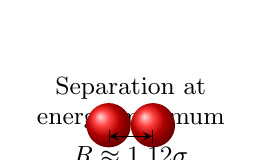
\begin{tikzpicture}
                \node[align=center, font=\small, text=black] (text) at (0, -1.2) {Separation at \\ energy minimum};

                \node[circle, minimum size=16pt, inner sep=0, shading=ball, ball color=red] (M1) at (-8pt, -1.48) {};
                \node[circle, minimum size=16pt, inner sep=0, shading=ball, ball color=red] (M2) at (8pt, -1.48) {};

                \draw[ |<->|, >=stealth] (-8pt, -1.62) -- (8pt, -1.62) node[midway, below, font=\small, text=black] {$R \approx 1.12\sigma$};
            \end{tikzpicture}};;

            \node[draw=gray!80, fill=gray!10, rounded corners, inner sep=8pt] (MinBox) at (axis cs:1.85, 0.7) {
            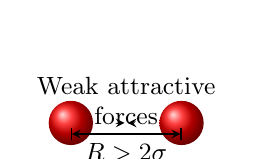
\begin{tikzpicture}
                \node[align=center, font=\small, text=black] (text) at (0, -1.2) {Weak attractive \\ forces};

                \node[circle, minimum size=16pt, inner sep=0, shading=ball, ball color=red] (M1) at (-20pt, -1.48) {};
                \node[circle, minimum size=16pt, inner sep=0, shading=ball, ball color=red] (M2) at (20pt, -1.48) {};

                \draw[ ->, >=stealth] (-0.08, -1.48) -- (-0.02, -1.48);
                \draw[ <-, >=stealth] (0.02, -1.48) -- (0.08, -1.48);
                \draw[ |<->|, >=stealth] (-20pt, -1.62) -- (20pt, -1.62) node[midway, below, font=\small, text=black] {$R > 2 \sigma$};
            \end{tikzpicture}};;
            \node[anchor=north] at (axis cs:0.8, -0.6) {repulsion};
            \node[anchor=north] at (axis cs:1.5, -0.6) {attraction};
            \end{axis}
        \end{tikzpicture}
        \label{fig1:Lennard Jones Potential}
        \caption{Lennard Jones Potential}
        \end{figure}

        The force exerted on $i$th atom by $k$th atom is given by the negative gradient of the interaction potential as follows,
        \begin{equation}
            \label{eq2: Force vector}
            \vec{f}_{k,i} = -\grad_{k,i}{u(r_{k,i})} = 24\epsilon \left[ 2\left(\frac{\sigma}{r_{k,i}}\right)^{12} - \left(\frac{\sigma}{r_{k,i}}\right)^{6}\right] \hat{r}_{i,j}
        \end{equation}

        The $x$ component is computed as,
        \begin{eqnarray}
            \label{eq3: Force along x direction}
            F_{x,i} & = & \sum_{k\neq i} f_{k,i} \cos{\theta_{k,i}} \\ \nonumber
            & = & \sum_{k\neq i} f_{k,i} \frac{x_i - x_k}{r_{k,i}} \\ \nonumber
            & = & 24 \epsilon \sum_{k\neq i} \frac{x_i - x_k}{r_{k,i}^2} \left[ 2\left(\frac{\sigma}{r_{k,i}}\right)^{12} - \left(\frac{\sigma}{r_{k,i}}\right)^{6}\right]
        \end{eqnarray}
        
        The $y$ component is computed as,
        \begin{eqnarray}
            \label{eq4: Force along y direction}
            F_{y,i} & = & \sum_{k\neq i} f_{k,i} \sin{\theta_{k,i}} \\ \nonumber
            & = & \sum_{k\neq i} f_{k,i} \frac{y_i - y_k}{r_{k,i}} \\ \nonumber
            & = & 24 \epsilon \sum_{k\neq i} \frac{y_i - y_k}{r_{k,i}^2} \left[ 2\left(\frac{\sigma}{r_{k,i}}\right)^{12} - \left(\frac{\sigma}{r_{k,i}}\right)^{6}\right]
        \end{eqnarray}

        \subsection{Time Integration: The Verlet Algorithm}
            To trace the trajectories, we must integrate Newton's second law, $m \ddot{x} = F(x)$, over discrete time steps $h$.

            \subsubsection{The Standard Verlet Algorithm}
            We can derive this via Taylor expansions of the position $x(t)$ moving forward and backward in time by $h$,
            $$x(t+h) = x(t) + h\dot{x}(t) + \frac{h^2}{2}\ddot{x}(t) + \frac{h^3}{6}x^{(3)}(t) + \mathcal{O}(h^4)$$
            $$x(t-h) = x(t) - h\dot{x}(t) + \frac{h^2}{2}\ddot{x}(t) - \frac{h^3}{6}x^{(3)}(t) + \mathcal{O}(h^4)$$
            Adding these two equations cleanly cancels out the odd-order velocity terms,
            $$x(t+h) + x(t-h) = 2x(t) + h^2\ddot{x}(t) + \mathcal{O}(h^4)$$
            The leading error term is $\mathcal{O}(h^4)$, indicating second-order accuracy. Substituting $\ddot{x}(t) = \frac{F(x(t))}{m}$, we get the explicit recursion relation:
            \begin{equation}
                \label{eq5: Position verlet (position)}
                x(t + h) = 2x(t) - x(t - h) + \frac{h^2}{m}F(x(t))
            \end{equation}
            We calculate $x(t - \Delta)$ using the relation:
            \begin{equation}
                \label{eq6: Position verlet (Previous position)}
                x(t - h) = x(t) - v(t) h + \frac{h^2}{m}F(x(t))
            \end{equation}
            Then the velocity can be derived from the position using central difference method as follows:
            \begin{equation}
                \label{eq7: Position verlet (derived velocity)}
                v(t + h) = \frac{x(t + h) - x(t - h)}{2 h}
            \end{equation}
            While this is time-reversible and conserves energy well, it has a severe flaw: it does not explicitly calculate velocity. This makes tracking the system's kinetic energy and temperature cumbersome.

            \subsubsection{The Velocity Verlet Algorithm}
            To resolve this, we decouple the second-order differential equation into two first-order equations: $\dot{x}(t) = v(t)$ and $\dot{v}(t) = \frac{F(x(t))}{m}$.
            We calculate the explicit position update using the standard Taylor expansion:
            \begin{equation}
                \label{eq8: Velocity verlet (Position Update)}
                x(t+h) = x(t) + hv(t) + \frac{h^2}{2m} F(x(t)) + \mathcal{O}(h^3)
            \end{equation}
            For the velocity, we use the forces at both the current and the newly calculated next step to update the velocity explicitly:
            
            $$v(t+h) = v(t) + \frac{h}{m} F(x(t)) + \frac{h^2}{2m} \left[\frac{F(x(t+h)) - F(x(t))}{h}\right] + \mathcal{O}(h^3)$$

            \begin{equation}
                \label{eq9: Velocity verlet (Velocity Update)}
                v(t+h) = v(t) + \frac{h}{2m} \left[F(x(t+h)) + F(x(t))\right] + \mathcal{O}(h^3)
            \end{equation}
            
            Both the Verlet and Velocity Verlet algorithms are symplectic integrators, meaning they preserve phase-space volume and exhibit long-term stability. However, their stability and accuracy depend on the choice of h:
            \begin{itemize}
                \item A smaller h improves accuracy but increases computational cost.
                \item A larger h can introduce numerical instability, leading to energy drift.
            \end{itemize}
            Overall, the Velocity Verlet algorithm is favored in molecular dynamics due to its superior handling of both position and velocity while maintaining second-order accuracy and stability.

        \subsection{Simulation Environment Boundaries and Units}
            \subsubsection{Periodic Boundary Conditions}
            Simulating a small number of particles (e.g., N = 25) is a rigid box introduces massive edge effects. We eliminate edges by wrapping the box into a torus topology. If a particles coordinate exceeds the box length $L_x$, we apply $x = x - L_x$. For pair interactions, we use the \textit{Minimum Image Convention}. This dictates that $i$th particle should only interact with the closest periodic image of $j$th particle.
            Let the raw displacement vector between $i$th and $j$th particle be:
            \begin{eqnarray*}
                dx & = & x_i - x_j \\
                dy & = & y_i - y_j
            \end{eqnarray*}
            The maximum possible physical separation between two interacting particles in this mapped space is exactly half the box length in either direction ($\frac{L_x}{2}$ and $\frac{L_y}{2}$). If the absolute calculated distance exceeds this, it means an image of $j$th particle in an adjacent periodic cell is actually closer to $i$th particle than the primary $j$th particle  itself.

            We correct the displacement vector components systematically:
            \begin{itemize}
                \item If $dx > \frac{L_x}{2}$, $j$th particle is too far "left", so we interact with its image on the "right": $dx = dx - L_x$.
                \item If $dx < -\frac{L_x}{2}$, $j$th particle is too far "right", so we interact with its image on the "left": $dx = dx + L_x$.
            \end{itemize}
            The same logic applies to the y-components:
            \begin{itemize}
                \item If $dy > \frac{L_y}{2}$, then $dy = dy - L_y$.
                \item If $dy < -\frac{L_y}{2}$, then $dy = dy + L_y$.
            \end{itemize}

            \subsubsection{Reduced Units}
            To avoid numerical underflow/overflow and make the code universally applicable, we non-dimensionalize the equations by setting $\sigma = 1$, $\epsilon = 1$, and $m = 1$. Consequently, time is measured in units of $\sigma \sqrt{m / \epsilon}$ (e.g., $\Delta t ^\prime = \frac{\Delta t}{\sigma \sqrt{m / \epsilon}}$).

    \section{Numerical Implementation}
        To build a clean, maintainable, and highly efficient Molecular Dynamics simulation, we constructed a modular architecture. Instead of single monolithic script, separating concerns into distinct modules ensures variables are safely scoped and physical routines are logically grouped.

        The simulation is divided into the following modules:
        \begin{enumerate}
            \item {\bf \texttt{md\_params}:} A global data repository containing precision definitions, system parameters (particle count, box dimensions), and dynamically allocated arrays for kinematics (position, velocity, force).
            \item {\bf \texttt{md\_init}:} This module handles the physical setup of the system, including placing particles on a spatial grid and assigning their initial thermodynamic states.
            \item {\bf \texttt{md\_forces}:} This module is designed to compute forces due to Lennard-Jones interaction and enforce \textit{Periodic Boundary Conditions}.
            \item {\bf \texttt{md\_integrator}:} Advances the system forward in time using the \textit{Velocity Verlet} algorithm.
            \item {\bf \texttt{md\_energy}:} Calculates the kinetic energy, potential energy of the system when the system reach thermal equilibrium.
            \item {\bf \texttt{md\_analysis}:} This module collects the velocities, generates the histogram, calculates $v_0$ from the average kinetic energy, and outputs the comparison data.
            \item {\bf \texttt{md\_main}:} The driver program that links the modules, executes the main time loop, and outputs data for visualization.
        \end{enumerate}
        \subsection{The Global Parameter Module (\texttt{md\_params})}
        First, we establish a robust data structure. Using double precision is critical in MD to prevent floating-point drift, especially when calculating the $r^{-12}$ repulsive term of the Lennard-Jones potential.
        \lstinputlisting[style= codestyle, label={lst:params}]{src/md_params.f90}

        \subsection{The Initialization Module (\texttt{md\_init})}
        To avoid infinite overlaps, we place the molecules in an $N_x \times N_y$ grid. To prevent the system from being perfectly crystalline, we introduce a small random spatial perturbation to each coordinate.
        
        For a particle $p$ mapped to grid indices $(i, j)$, the initial positions are:
        \begin{eqnarray*}
            x_p = \frac{L_x}{N_x}(i - 0.25 \times \text{rand}) \\
            y_p = \frac{L_y}{N_y}(j - 0.25 \times \text{rand})
        \end{eqnarray*}
        where $\text{rand}$ is a uniform random number in the interval $[0, 1)$.

        We assign initial velocities drawn from a uniform random distribution ranging from $[-0.5 v_{initial}, 0.5 v_{initial}]$. If we assign velocities purely randomly, the net momentum of the system will likely be non-zero, causing the entire container of gas to drift. To prevent this, we must ensure the Center of Mass (COM) velocity is strictly zero.
        
        Let the total momentum be $\vec{P} = \sum_{i=1}^{N_{mol}} m_i \vec{v}_i$. Because we are operating in reduced units where $m_i = 1$, the COM velocity is simply the arithmetic mean of the individual velocities:$$\vec{V}_{COM} = \frac{1}{N_{mol}} \sum_{i=1}^{N_{mol}} \vec{v}_i$$
        To eliminate drift, we apply a Galilean transformation, shifting the reference frame to the center of mass by subtracting $\vec{V}_{COM}$ from every particle's velocity:$$\vec{v}_i' = \vec{v}_i - \vec{V}_{COM}$$
        \lstinputlisting[style= codestyle, label={lst:init}]{src/md_init.f90}

        \subsection{The Forces Module (\texttt{md\_forces})}
        To calculate forces, we first calculate the displacement between $i$th and $j$th particle using \textit{Minimum Image Convention} we discussed earlier. Once we have the minimum image displacement $(dx, dy)$, the squared distance is simply $r^2 = dx^2 + dy^2$. The force calculation will be according to equation (\ref{eq3: Force along x direction}) and (\ref{eq4: Force along y direction}).

        Computationally, calculating high-order powers (like $r^{12}$) or square roots is extraordinarily expensive. We can optimize this rigorously by working entirely in squared inverse terms. Because we are using reduced units where $\sigma = 1$ and $\epsilon = 1$, the calculation collapses beautifully.

        Let us define an intermediate variable for the inverse squared distance: $$t_1 = \frac{1}{r^2}$$
        We can obtain the higher order terms through simple multiplication: $$t_2 = (t_1)^3 = \frac{1}{r^6}$$
        The magnitude of the force vector becomes: $$F_{scalar} = 24 \cdot t_1 \cdot (2 t_2^2 - t_2)$$
        The force components are then simply $F_x = dx \cdot F_{scalar}$ and $F_y = dy \cdot F_{scalar}$.
        
        By Newton's Third Law, the force particle $i$ exerts on $j$ is equal and opposite to the force $j$ exerts on $i$ ($\vec{F}_{ji} = -\vec{F}_{ij}$). We can cut our computational load in half by looping $i$ from $1$ to $N_{mol}-1$ and $j$ from $i+1$ to $N_{mol}$, applying the computed force to $i$ and its negative to $j$ simultaneously.
        \lstinputlisting[style= codestyle, label={lst:forces}]{src/md_forces.f90}

        \subsection{The Integrator Module (\texttt{md\_integrator})}
        To advance the system forward in time, we implement the \textit{Velocity Verlet} algorithm as discussed in equation (\ref{eq8: Velocity verlet (Position Update)}) and (\ref{eq9: Velocity verlet (Velocity Update)}). To calculate the new velocity $v(t+h)$, we strictly require the new force $F(x(t+h))$. Therefore, the order of operations in our code must be precisely sequenced:
        \begin{enumerate}
            \item {\bf Advance Positions:} Calculate $x(t+h)$ and $y(t+h)$ using current velocities and current forces.
            \item {\bf Enforce Boundaries:} Immediately apply \textit{Periodic Boundary Conditions} to the new positions to ensure particles don't escape the simulation box.
            \item {\bf Store Old Forces:} Save the current forces ($F(x(t))$) into temporary arrays ($Fx1$, $Fy1$) because we are about to overwrite them.
            \item {\bf Update Forces:} Call \texttt{calculate\_forces()} subroutine to compute the new forces $F(x(t+h))$ based on the newly updated positions.
            \item {\bf Advance Velocities:} Calculate $v(t+h)$ using the stored old forces and the newly computed forces.
        \end{enumerate}
        \lstinputlisting[style= codestyle, label={lst:integrator}]{src/md_integrator.f90}

        \subsection{The Energy Module (\texttt{md\_energy})}
        This module is created specifically for tracking the thermodynamics of the system. While calculating forces and potential energy in the same loop is computationally faster, keeping them separate increase the maintainability.
        \lstinputlisting[style= codestyle, label={lst:energy}]{src/md_energy.f90}

        \subsection{The Analysis Module (\texttt{md\_analysis})}
        To verify the simulation is physically accurate, we must prove that the steady-state velocities of the argon atoms obey the Maxwell-Boltzmann distribution.

        The exact 2D Maxwell-Boltzmann speed distribution is: 
        \begin{equation}
            \label{eq10: MB Distribution Exact}
            P(v) = \frac{m}{k_B T} v e^{-\frac{mv^2}{2k_B T}}
        \end{equation}
        In the simulation's reduced units, mass $m=1$. By the Equipartition Theorem in 2D, the average kinetic energy per particle is $\langle KE \rangle = \frac{2}{2} k_B T = k_B T$. Therefore, the most probable velocity $v_0$ satisfies $v_0^2 = k_B T$. Substituting this to equation (\ref{eq10: MB Distribution Exact}) yields: 
        \begin{equation}
            \label{eq11: MB Speed Distribution}
            P(v) = \frac{v}{v_0^2} e^{-0.5 \left(\frac{v}{v_0}\right)^2}
        \end{equation}

        To compare the discrete simulation data against this continuous theoretical curve, we must construct a normalized histogram:
        \begin{enumerate}
            \item {\bf Equilibration:} The system initially exhibits transient, non-physical behavior as the grid arrangement breaks down. We only sample velocities after a designated equilibrium time (e.g., $t > 10000$ steps).
            \item {\bf Binning:} We divide the range of observed speeds into discrete bins of width $h$. We count how many times a particle's speed falls into each bin.
            \item {\bf Normalization:} The raw counts must be divided by the total number of samples and the bin width $h$ to represent a probability density function. A highly accurate way to find the total integration area of the discrete data is using Simpson's 1/3 Rule.
        \end{enumerate}
        \lstinputlisting[style= codestyle, label={lst:analysis}]{src/md_analysis.f90}

        \subsection{The Main Program (\texttt{md\_main})}
        Since all the modules are defined above, we can write the main driver. This program will \texttt{use} all the modules, initialize the system, run the \textit{Velocity Verlet} time loop, and output the energy data to track the conservation of energy along with the velocity distribution analysis.
        \lstinputlisting[style= codestyle, label={lst:main}]{src/md_main.f90}
        
    \section{Results and Discussion}
        The molecular dynamics simulation was executed over $N_{step} = 100,000$ time steps with a reduced time step of $\Delta t = 0.01$. To investigate finite-size effects and the emergence of macroscopic thermodynamics, the simulation was performed for two distinct system sizes: a baseline model of $N=25$ atoms in a $20 \times 20$ box, and an expanded model of $N=100$ atoms in a $40 \times 40$ box. The box dimensions were dynamically scaled to ensure the number density ($\rho = 0.0625$) remained strictly constant across both simulations.

        \subsection{Spatial Evolution: Initial and Final States}
        At the start of the simulation ($t=0$), particles were placed in a perfect grid ($5 \times 5$ for $N=25$, and $10 \times 10$ for $N=100$) to prevent infinite repulsive forces from overlapping coordinates, and were assigned random initial velocities.
        
        By the end of the simulation ($t=100,000$), the spatial distribution of the particles had completely randomized. The initial ordered grid structure "melted" as the systems evolved into chaotic, gas-like states. The comparative final-state quiver plots visually highlight the scale difference between the two systems. While the 25-particle system exhibits large empty voids characteristic of a highly confined microstate, the 100-particle system demonstrates a much more uniform spatial distribution. This visual evidence reinforces that the larger system behaves more like a continuous thermodynamic fluid, properly representing a well-mixed gas.
        \begin{figure}[H]
            \centering
            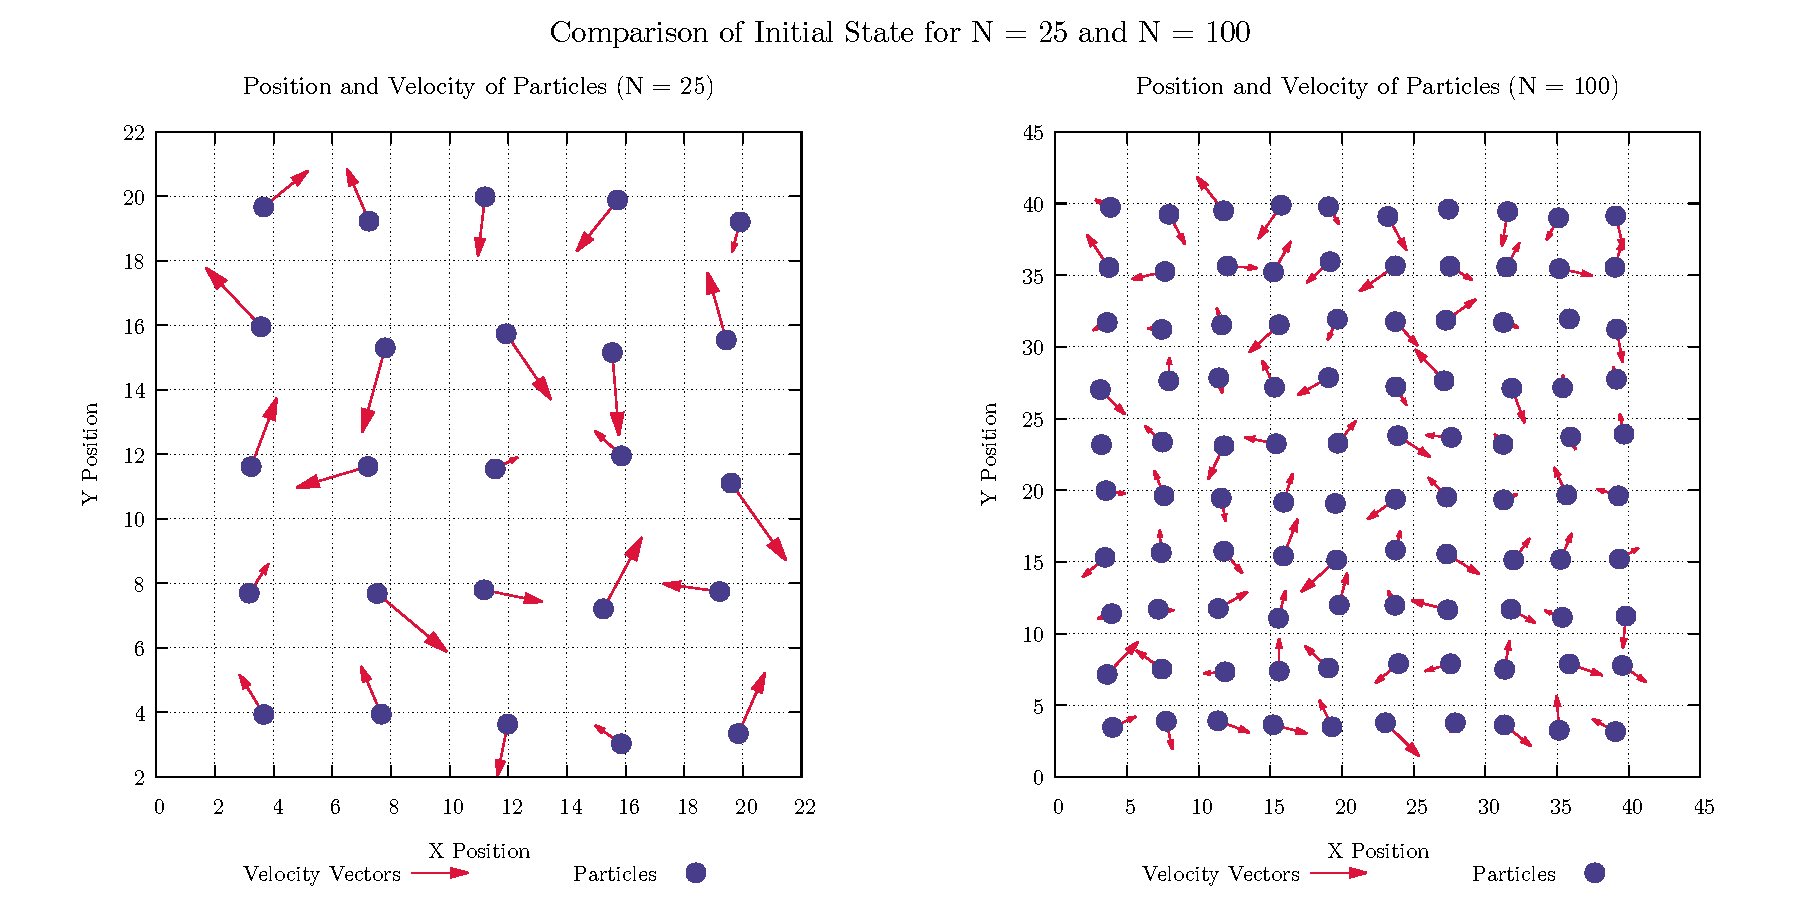
\includegraphics[width=0.99\textwidth]{plots/Initial.pdf}
            \label{fig2:Initial_state}
        \end{figure}
        
        \begin{figure}[H]
            \centering
            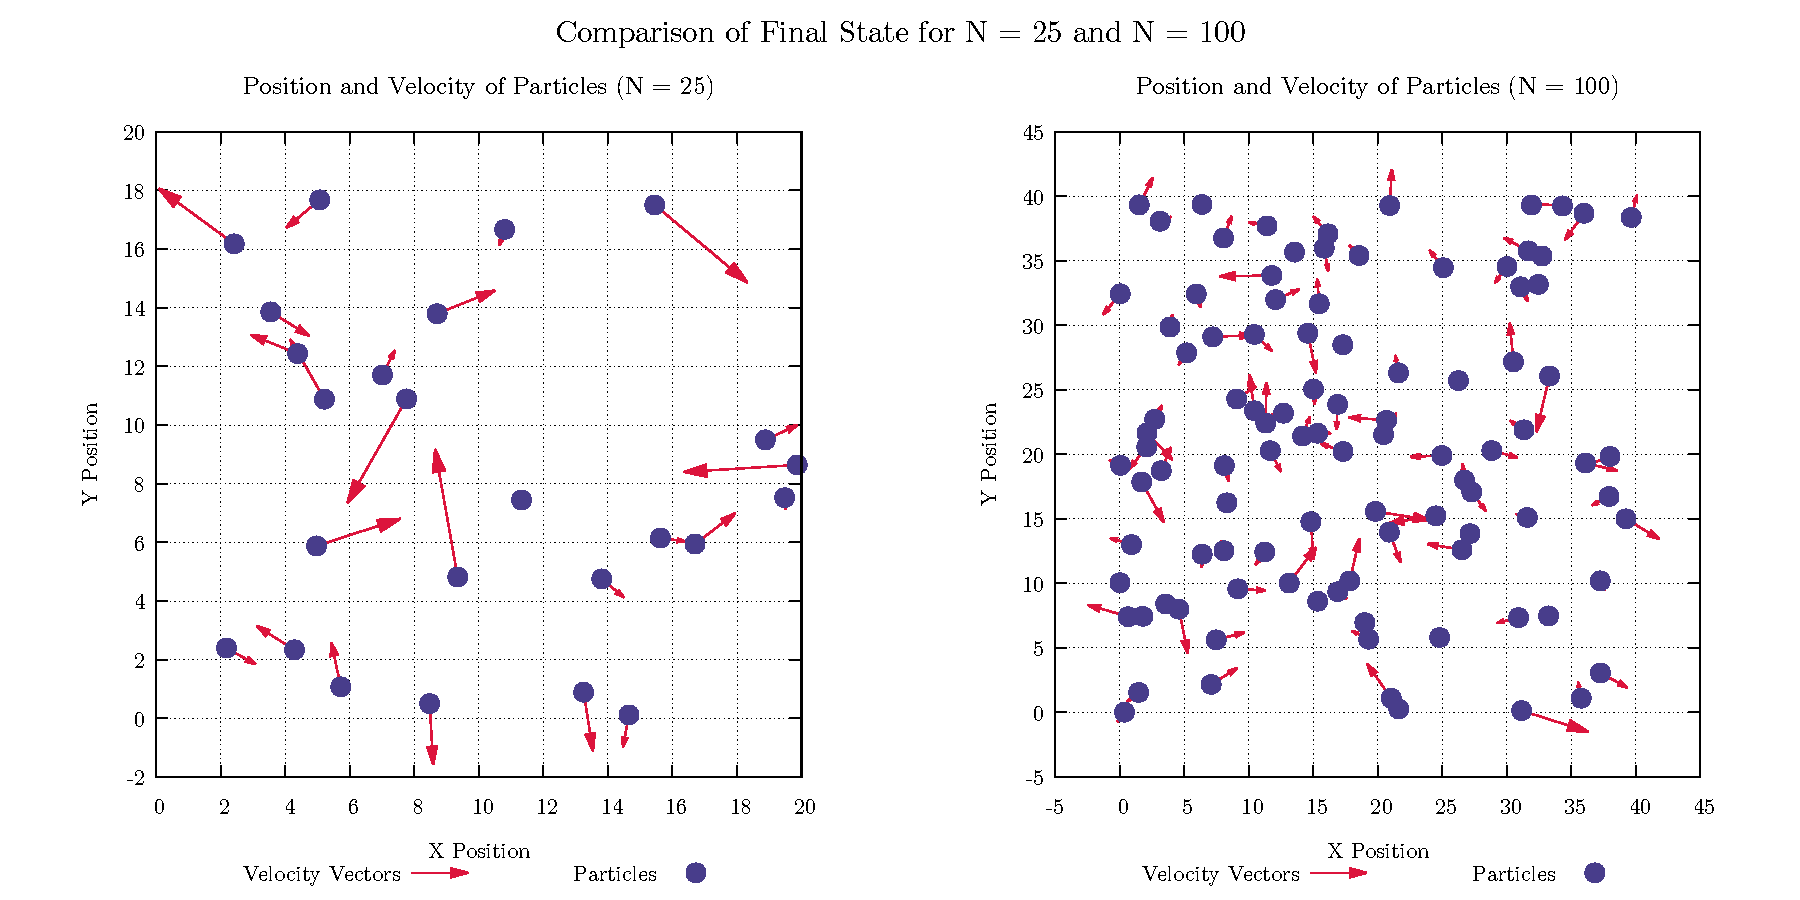
\includegraphics[width=0.99\textwidth]{plots/Final.pdf}
            \label{fig3:Final_state}
        \end{figure}
        
        \subsection{Conservation of Energy}
        Because the simulated system is strictly isolated, classical mechanics dictates that the total energy must remain constant. The energy time-series plots for both $N=25$ and $N=100$ confirm this fundamental principle, displaying a perfectly flat horizontal line for the total energy throughout the entire 100,000-step integration.
        
        While the total energy remained constant, the kinetic and potential energies exhibited continuous, dynamic fluctuations. The data reveals a perfect counter-balancing relationship: every localized increase in kinetic energy is met with an identical decrease in potential energy (and vice versa).
        
        Furthermore, comparing the two systems demonstrates that energy is an extensive thermodynamic property. The total energy of the $N=25$ system stabilized at approximately 55 reduced units, whereas the $N=100$ system stabilized at roughly 220 reduced units. Quadrupling the number of particles directly quadrupled the total energy, perfectly aligning with theoretical expectations.
        \begin{figure}[H]
            \centering
            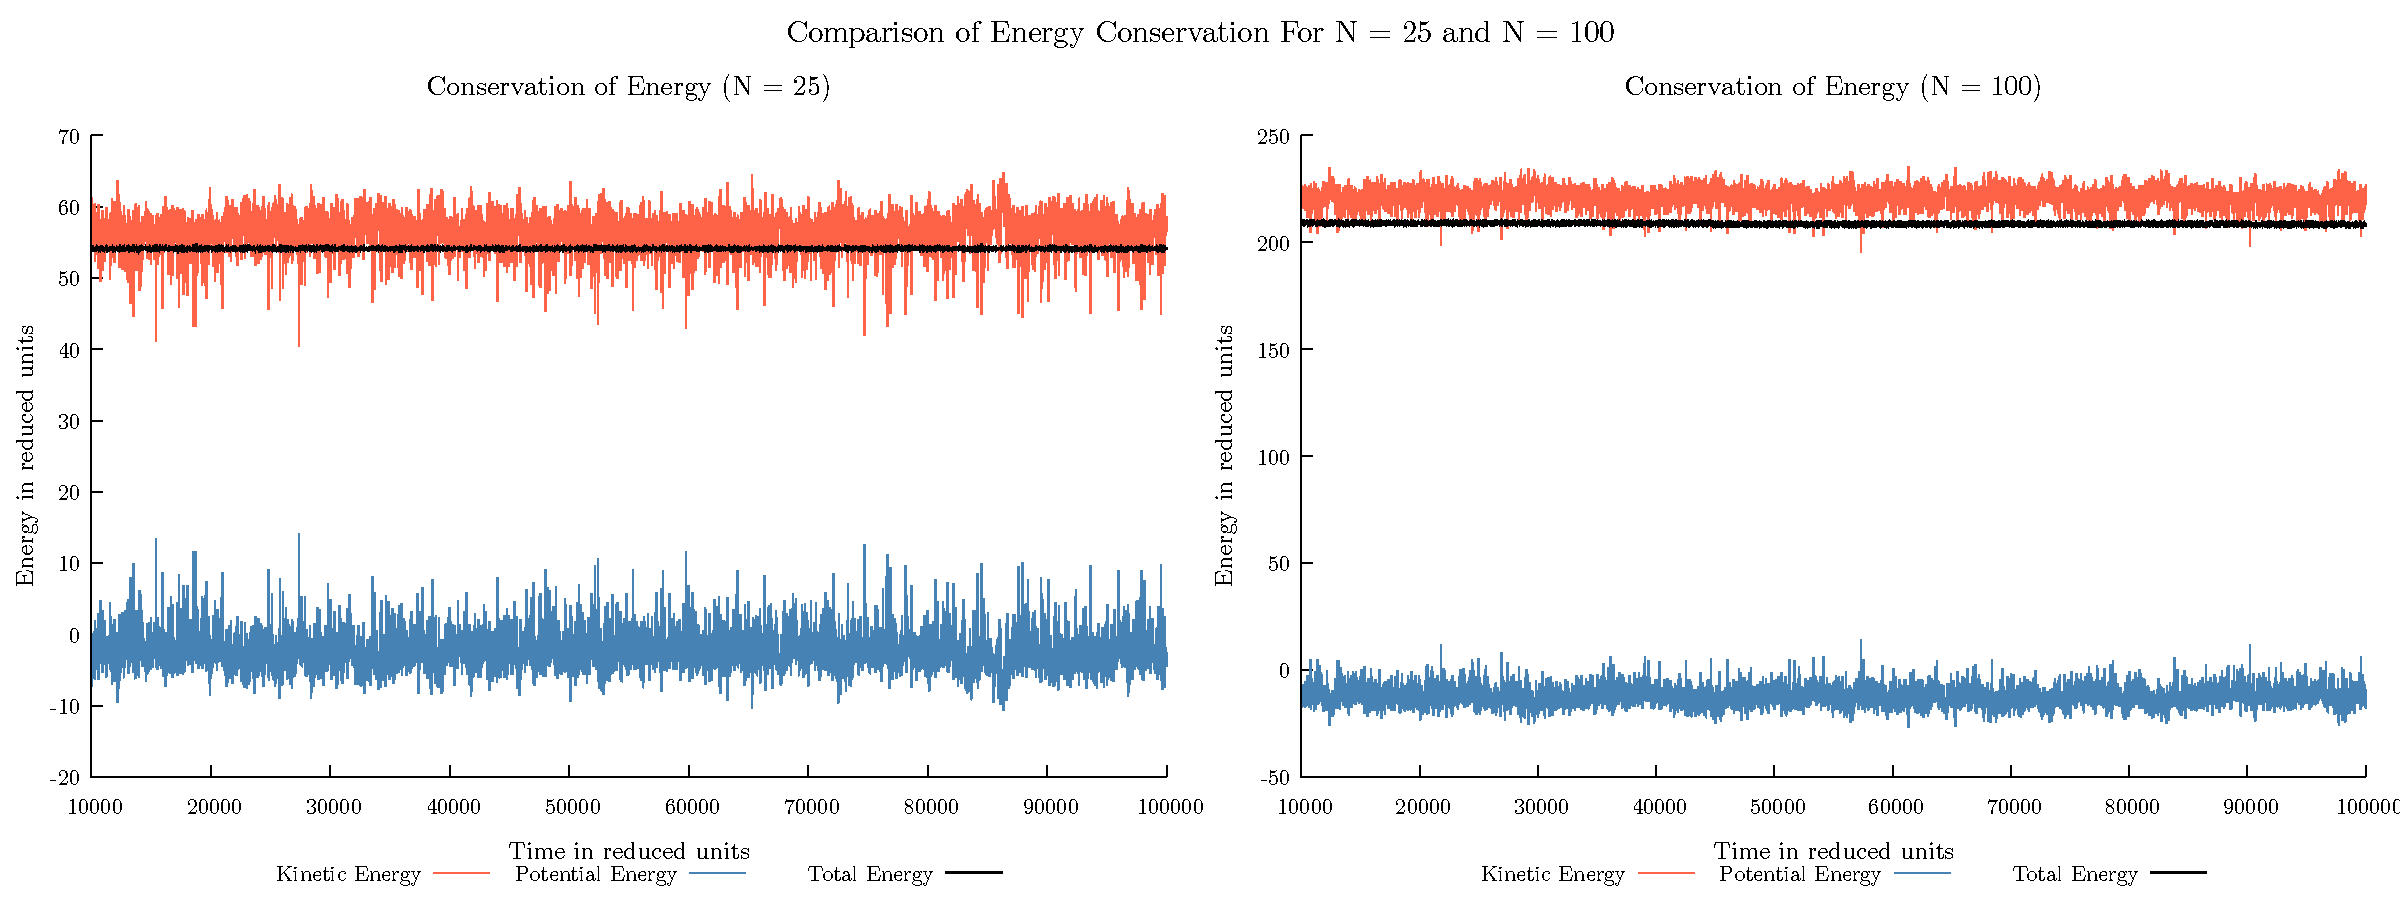
\includegraphics[width=1.0\textwidth]{plots/Energy.pdf}
            \label{fig4:Energy}
        \end{figure}
        
        \subsection{Velocity Distribution and the Thermodynamic Limit}
        To verify that the systems reached thermal equilibrium, the simulated velocities were sampled and compiled into histograms using 1,000 bins. These were plotted against the continuous theoretical 2D Maxwell-Boltzmann distribution, calculated using both the most probable velocity ($V_{most}$) and the root-mean-square velocity derived from the average kinetic energy ($\sqrt{KE_{avg}}$).

        The side-by-side comparison of the velocity distributions provides a striking demonstration of the \textbf{thermodynamic limit}.
        \begin{itemize}
            \item For the $N=25$ system, the velocity histogram is highly jagged and noisy. Because it is a small microcanonical ensemble, it is highly susceptible to statistical fluctuations, fitting only loosely around the theoretical Maxwell-Boltzmann curve.
            \item For the $N=100$ system, the law of large numbers heavily mitigates these statistical anomalies. The expanded system's histogram fills in the gaps and smoothly hugs the theoretical probability density function.
        \end{itemize}

        \begin{figure}[H]
            \centering
            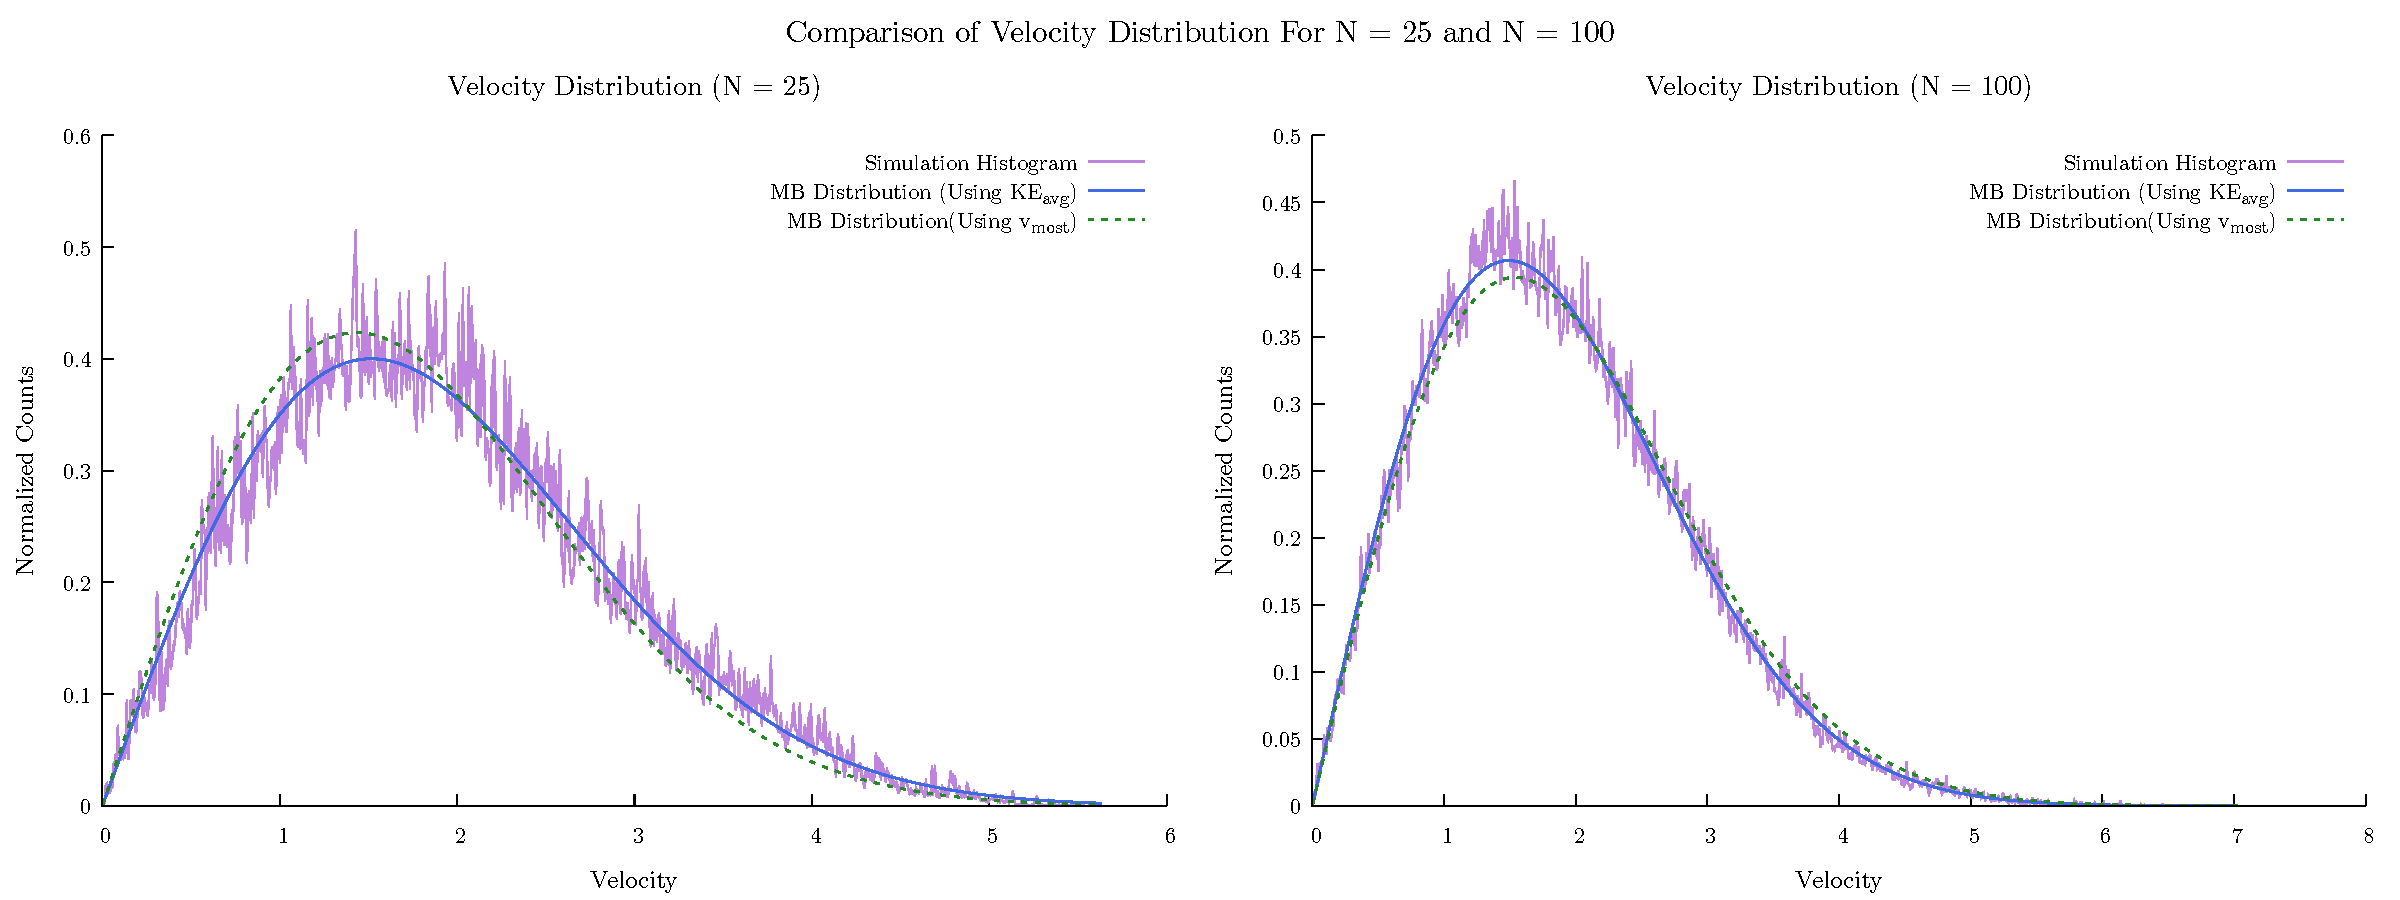
\includegraphics[width=1.0\textwidth]{plots/Velocity_dist.pdf}
            \label{fig5:Velocity Distribution}
        \end{figure}

        This statistical convergence proves that while small numerical models can simulate basic Newtonian trajectories, larger particle counts are required to suppress microscopic fluctuations and accurately extract macroscopic thermodynamic observables.

    \section{Conclusion}

        This study successfully implemented a modular molecular dynamics simulation in Fortran 90, utilizing the velocity Verlet algorithm to accurately model the motion of argon atoms under the Lennard-Jones potential. The numerical results unequivocally validated the core physical principles governing isolated classical systems. Most notably, the total energy of the system remained strictly conserved over 100,000 time steps. The continuous fluctuations in kinetic and potential energy exhibited a perfect counter-balancing relationship, ensuring thermodynamic stability throughout the integration process.Furthermore, by extracting macroscopic observables from the microscopic atomic trajectories, the simulation successfully reproduced the theoretical 2D Maxwell-Boltzmann velocity distribution. The extension of the simulation from $N=25$ to $N=100$ particles provided a compelling visual and statistical demonstration of the thermodynamic limit. While the 25-atom system exhibited the expected statistical noise of a small microcanonical ensemble, the 100-atom system drastically reduced these fluctuations, adhering tightly to the theoretical probability density function and visually representing a continuous, well-mixed gas.Overall, this computational model effectively captured the microscopic interactions of atomic particles, proving the reliability of the velocity Verlet method and demonstrating how macroscopic thermodynamic equilibrium emerges directly from deterministic Newtonian mechanics.

\end{document}